\documentclass[conference]{IEEEtran}

% Package list
\usepackage{graphicx}
\usepackage{fancyref}
\usepackage[utf8]{inputenc}
\usepackage[backend=biber,
  bibstyle=ieee,
  citestyle=numeric-comp,
  sortcites=true]{biblatex}
\usepackage[pdftex,
  pdfauthor={Name},
  pdftitle={Title},
  pdfsubject={Computer Science},
  pdfkeywords={Parallel},
  pdfcreator={latexmk}]{hyperref}

% import references
\addbibresource{references.bib}
% Graphics path
\graphicspath{{images/}}
% Section path
\makeatletter
\def\input@path{{sections/}}
\makeatother

% Title
\title{Title}

% Author(s)
\author{\IEEEauthorblockN{Name}
\IEEEauthorblockA{
UiT The Arctic University of Norway\\
Department of Computer Science\\
Email: xxxXXX@post.uit.no}}
% \and
% \IEEEauthorblockN{name}
% \IEEEauthorblockA{
% UiT The Arctic University of Norway\\
% Department of Computer Science\\
% Email: email@uit.no}
% \and
% \IEEEauthorblockN{name}
% \IEEEauthorblockA{
% UiT The Arctic University of Norway\\
% Department of Computer Science\\
% Email: email@uit.no}}

\begin{document}
\maketitle
\begin{abstract}
  This is a scientific paper.
\end{abstract}
\section*{Introduction}
\textbf{Introduction from \cite{Dijkstra} Paper}\\
Given in this paper is a solution to a problem for which,
to the knowledge of the author, has been an open question
since at least 1962, irrespective of the solvability. The
paper consists of three parts: the problem, the solution,
and the proof. Although the setting of the problem might
seem somewhat academic at first, the author trusts that
anyone familiar with the logical problems that arise in
computer coupling will appreciate the significance of the
fact that this problem indeed can be solved.\cite{Dijkstra}
\section*{Design}
\textbf{Text fetched from \cite{Usgvs} web page}\\
The Data Grapher can plot one or two time-series datasets from a single site, either as a time-series graph or an XY graph. Here is an example of a time-series graph of oxygen percent saturation and water temperature from a site in Oregon:\cite{Usgvs}
\begin{figure}[h]
  % \textwith is the width of the whole A4 sheet, and since we use double column we need to scale the image down.
  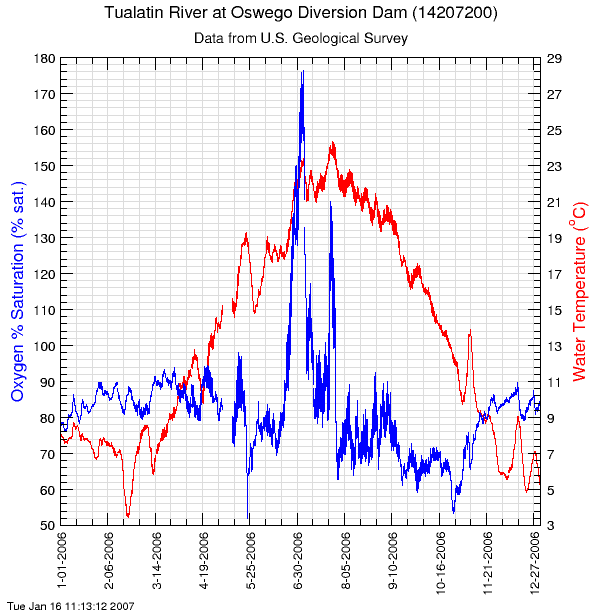
\includegraphics[width=0.5\textwidth]{example.png}
  \caption{\href{https://or.water.usgs.gov/grapher/tutorial/examples.html}{link here}}
\end{figure}

\section*{Discussion}
\textbf{Example Table}\\
\begin{center}
  \begin{tabular}{| l | c | r |}
    \hline
    \textbf{proc} & \textbf{nodes} & \textbf{time} \\
    \hline
    5  & 5 & 2 min. 45 sek. \\
    10 & 5 & 2 min. 15 sek. \\
    15 & 5 & 1 min. 45 sek. \\
    20 & 5 & 1 min. 15 sek. \\
    \hline
  \end{tabular}
\end{center}

\section*{Experimental setup}
\textbf{Example tools}\\
Profiling tools used:
\begin{enumerate}
  \item \textit{gproof}
  \item \textbf{valgrind}
  \item vampir
\end{enumerate}

\section*{Conclusion}
 $f(x) = 2x + 4$ \\
$$f(x) = 2x + 4$$\\
\section*{Evaluation}


% Print bibliography
\printbibliography
\end{document}
